\newpage
\section{Inter-Model Consistency Checking with TGGs}
\hypertarget{sec:cc}
\genHeader

TGGs can also be used to \emph{check consistency} between a source and target model.
In this case, correspondences and a protocol for consistent parts of the models are created.
Inconsistent parts can optionally be saved as delta (which again can be propagated again via model synchronization).

eMoflon solves an optimization problem over TGGs to detect \emph{maximum consistent portions} of two models.
You therefore need to install the Gurobi optimizer (\url{http://www.gurobi.com/}) for which free academic licences are available.
Next, you need to involve Gurobi in your integration project:

\begin{stepbystep}
\item Navigate to the Java Build Path properties of your integration project and set the native library location for system libraries to the \texttt{bin} folder of your Gurobi installation (\Cref{eclipse:gurobiNative}).

\begin{figure}[htbp]
\renewcommand\figurename{Figure}
\begin{center}
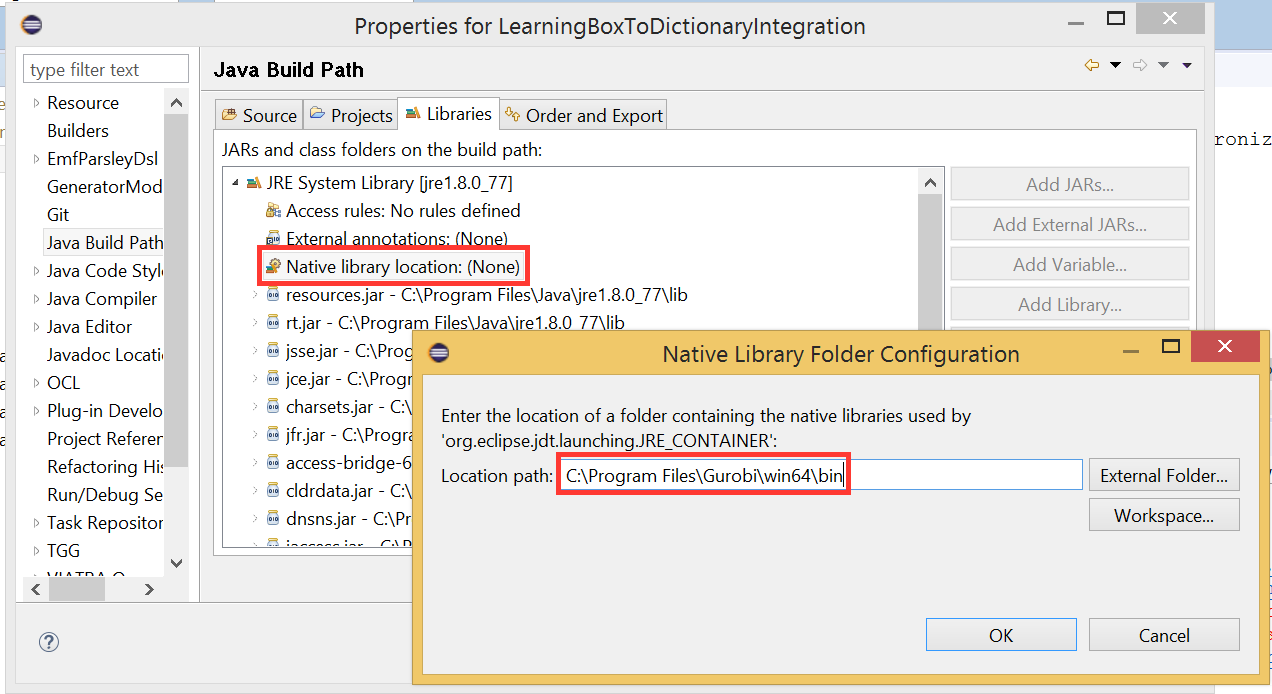
\includegraphics[width=0.65\textwidth]{nativeLibrary.png}
\caption{Add Gurobi to your native library location}
\label{eclipse:gurobiNative}
\end{center}
\end{figure}

\item Add \texttt{gurobi.jar} in the \texttt{lib} folder of your Gurobi installation as an external JAR to your integration project (\Cref{eclipse:externalJar}).

\begin{figure}[htbp]
\renewcommand\figurename{Figure}
\begin{center}
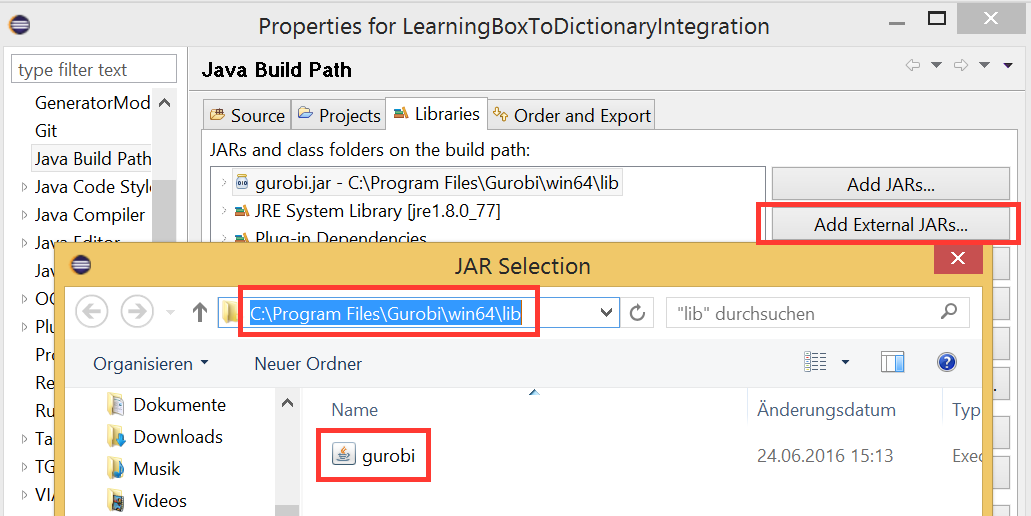
\includegraphics[width=0.65\textwidth]{externalJar.png}
\caption{Add gurobi.jar to your integration project}
\label{eclipse:externalJar}
\end{center}
\end{figure}
\end{stepbystep}

Open \javaCode{LearningBoxToDictionaryIntegrationConsistencyCheck.java} in the \texttt{src} folder of your project (\Cref{eclipse:ccstub}).
By analogy to the model transformation and synchronization stubs, this class loads your models, performs a consistency check, prints info in the console about the consistency of your models, and saves the resulting correspondences as well as the protocol.
The Boolean \javaCode{prepareDeltas} indicates whether the inconsistent elements in your source and target models should be shifted to a delta model (empty deltas will be saved if your models are completely consistent).
If deltas are prepared, the source and target models will be reduced to their consistent portions, i.e., they will potentially be changed (we thus recommend, as done in the stub, to save all results in some other path than your original models).
Finally, note that the prepared deltas can then be propagated using forward and backward synchronization as discussed in previous sections.

\begin{figure}[htbp]
\renewcommand\figurename{Figure}
\begin{center}
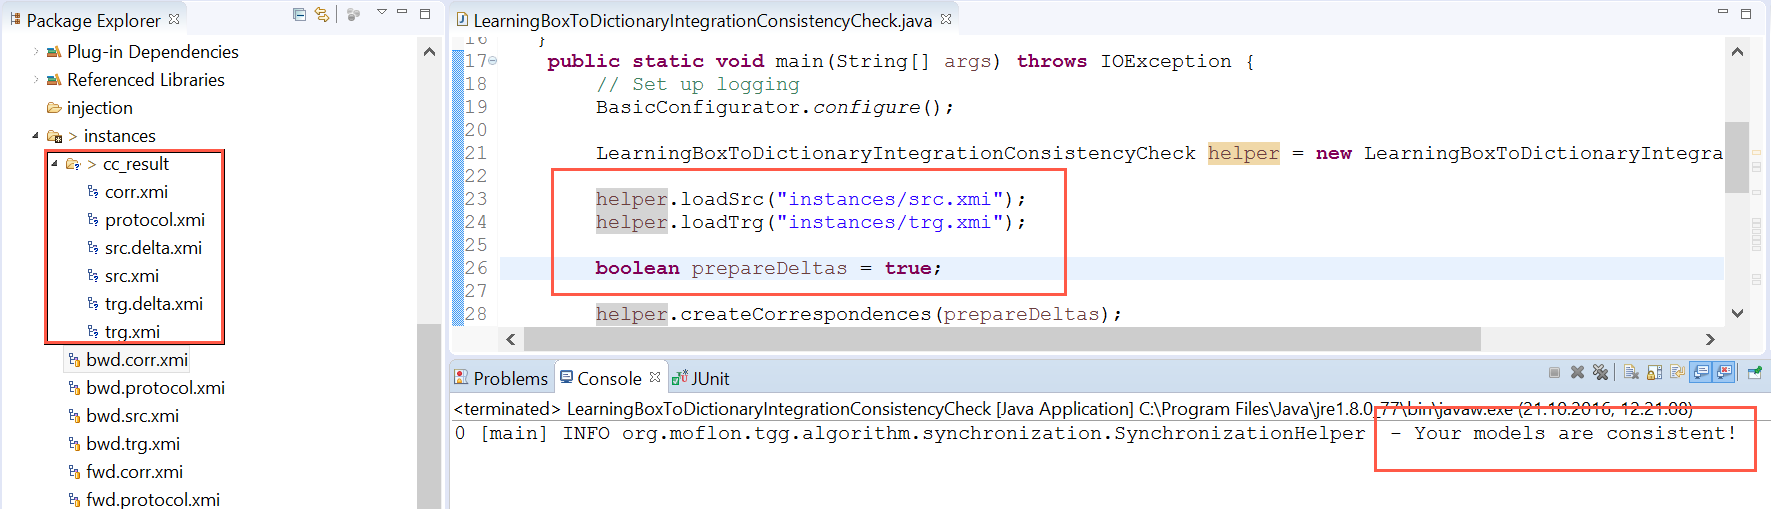
\includegraphics[width=1\textwidth]{ccstub.png}
\caption{The stub class for consistency checking}
\label{eclipse:ccstub}
\end{center}
\end{figure}

